\documentclass[lang=cn,cite=super]{elegantpaper}
\usepackage{bm,appendix,graphicx,float,booktabs,babel,makecell,natbib,longtable,tabularx}
\renewcommand{\bibsection}{}
\title{低成本普惠型智能家居方言指令转换器的研究}
\author{陶理}
\date{}

\begin{document}
\maketitle
\begin{abstract}
    本研究探讨了低成本普惠型智能家居方言指令转换器的设计与实现。通过建立包含普通话和多种方言的智能家居语音指令数据库,利用梅尔频率倒谱系数(MFCCs)和奇异值分解(SVD)等算法,提取并降维音频特征,构建了方言指令转换模型。该模型通过回归算法计算方言与普通话指令之间的映射关系,并采用计算余弦相似度的方式预测方言指令的含义。实验结果表明,该方法在减少算力消耗和数据需求的同时,能够有效识别多种方言的智能家居语音指令,具有较高的转换准确率。本研究为智能家居方言用户提供了一种便捷的语音控制解决方案,并为方言的保护和应用提供了新的技术支持。
    \keywords{智能家居, 语音识别, 方言语音指令转换, 梅尔频率倒谱系数, 奇异值分解}
\end{abstract}
\setcounter{section}{-1}
\section{引言}
随着普通话的推广,为了更好地与各族人民交流,方言的盛行注定会成为过去时。不过,各地迥异的方言是中华民族传承千年的瑰宝。以吴语为例:现如今普通话已经只剩下四个声调,即所谓的阴平、阳平、上声、去声,但是在古汉语中还有一个声调为入声,在古诗文的韵律中时常出现;如在浙江义乌话中,声调达到了10个。因为有入声,所以使用方言阅读古诗文能够接近古人在创作时的读音,相较于普通话更有韵味。全中国共有约10种方言大类,如图\ref{fig:chinese-lanaguages-map}所示,其中包括吴语、粤语等.而各地区又有不同的发音、措辞上也有区别,如在浙江,由于丘陵地势,不同地域的交流不频繁,使得同属吴语系的发音天差地别。
\begin{figure}[h]
    \caption{\label{fig:chinese-lanaguages-map}主要方言分布地图}
    \centering
    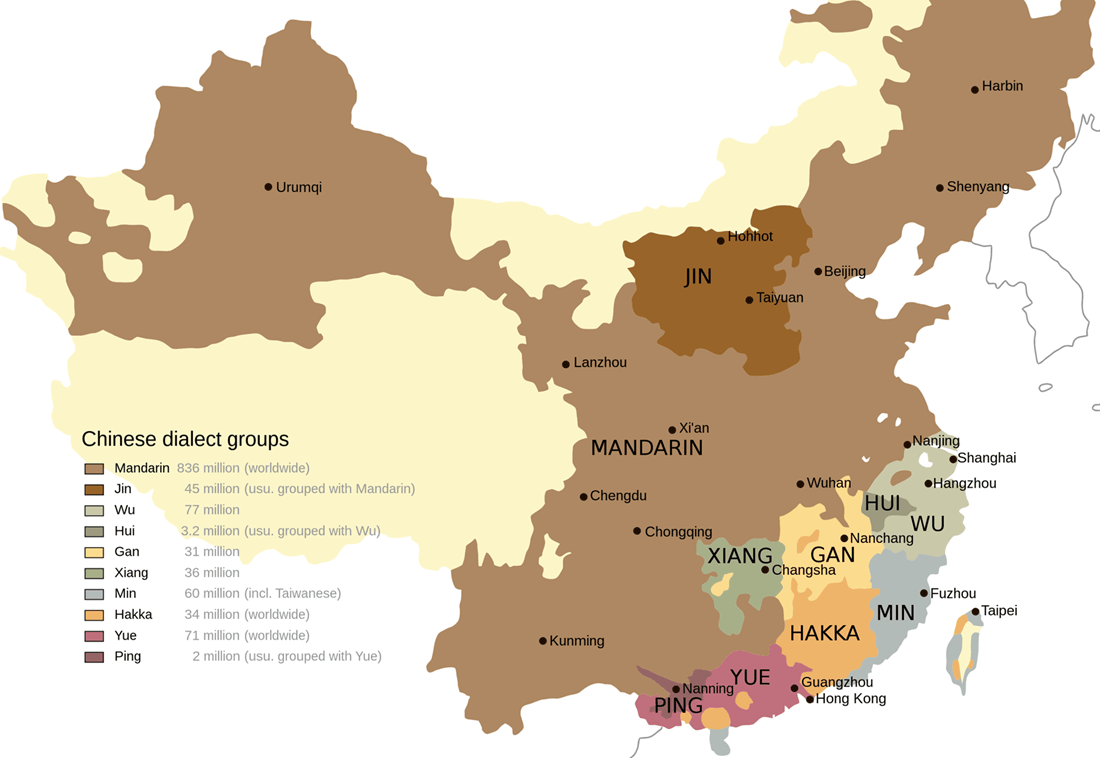
\includegraphics[scale=0.3]{chinese-lanaguages-map.png}
\end{figure}

方言的多样性也同样是方言在文化上重要性的体现。但是如今的方言正在高速消亡,多样性在飞速下降,特别是小众方言。沪剧、川剧、粤语歌曲等流行的艺术形式使得大方言得到了一定程度上的新生。但是还是存在根本性的问题:在这些方言流行的地域上,新一代的年轻人同样大多都说普通话,若是没有进一步的保护措施,方言将很快走下历史的舞台。早在2005年的11月,时任教育部语言文字信息管理司司长李宇明在接受《语言文字周报》采访时,他指出:“建立和谐的语言生活,首先要对语言多样性有充分的认识,要尊重各民族的方言,要尊重各种方言,包括尊重繁体字等历史上的文字,因为这些都是中华民族的宝贵财富。”

因此,虽然方言的小众化是不可逆的,但是及时的研究能够更多地保留这一非物质文化遗产。因此需要尽快进行研究。
吴永焕\cite{WuYonghuan}就方言的保护在必要性和紧迫性的方面进行了论证,强调了要抢记方言资料,尽可能延缓方言特征消失速度;
黄涛\cite{Huangtao}强调了方言在文化价值上的重要性;相应的保护政策也相继出台,因而保护方言是很有必要的。

另外,在高度信息化的现代社会,语音识别正在被广泛地应用和推广。语音识别技术使得人们可以方便地通过语音来交流、控制和感知信息。由于方言的发音和说话习惯与普通话大相径庭,因此使用普通话数据训练得到的语音识别模型无法准确地预测方言语音的含义。这会导致两个后果:
\begin{enumerate}
    \item 方言的使用场景减少
    \item 说方言的用户无法使用基于语音识别的各种设施。
\end{enumerate}

智能家居是以语音识别为基础,智能家具通过语音模型理解人的指令。但是目前模型的缺陷在于其大多基于普通话进行训练,因此对于方言的识别精度很低。而在方言识别领域,如今只有大方言的语音识别模型,科技公司出于对于利益的考量,并没有大量资本投入小众方言的研究,因此小众方言并没有对应的语音识别模型。这导致说小众方言的使用者只能使用普通话进行语音控制。而小众方言的使用者占我国总人数的很大比重。并且,不会说普通话的人群大多未老年人,而老年人正应该是便捷服务的享受者。因此针对小众方言研究方言指令转换器是十分有必要的。

在此之前,已经有许多学者就方言识别进行了研究:
武瑞丰\cite{WuRuiFeng}提出了人工智能在方言建档中有很大的作用和优点;
王岐学、钱盛友\cite{WangQiXue}等利用梅尔频率倒谱系数(MFCCs)对湖南方言进行特征提取,并利用差分特征和高斯混合模型进行模式识别;
石佳影、黄威\cite{ShiJiaYing2016}利用梅尔倒谱系数(MFCCs)对四川方言进行特征提取,并使用了基于Kaldi平台的深度神经网络(DNN),构建了基于语音与普通话的四川方言语料库;
杨波\cite{YangBo2019}构建了循环神经网络(RNN)为基础的声学模型,并以此搭建了桂柳方言的语音识别系统;
张宇聪\cite{ZhangYuCong2016}分别运用了隐马尔科夫模型(HMM)和长短时记忆模型(LSTM)构建了语音识别模型和藏语声学特征提取器,并以此完成了藏语语音识别系统;
余陆峰\cite{YuLuFeng2019}使用多种深度学习算法,并利用TensorFlow框架进行实现,最终对比得出了效果最佳的关于客家方言的语音识别系统;
徐凡、杨剑峰等\cite{XuFan2021}基于自注意力的端到端模型,设计了方言语音识别系统;
刘林泉等人\cite{LiuLinQuan2008}采用基于距离度量的识别基元扩展方法设计了小样本量的上海话方言识别系统;
杨奭喆\cite{YangShiZhe2020}和彭煦潭等\cite{peng2020}\cite{2021Cross}分别均利用“无监督跨语言词向量”的算法,分别研究了12种不同的语言并构建了语音识别系统。

前人的研究受限于所用算法对于数据量的要求,需要花费大量方言语音数据。本研究旨在通过小数据量的方言数据,构建方言语音指令转换器,利用特征值提取算法,建立方言指令音频数据特征向量矩阵,并通过数学模型寻找目标方言和普通话的向量之间的映射关系,将目标方言的语音指令的特征向量矩阵映射至普通话的特征向量矩阵,并采用计算余弦相似度的方式预测方言指令的含义。

\section{智能家居语音指令数据库}

为了更好地支持智能家居语音指令的识别和理解,我们构建了一个包含普通话和多种方言的智能家居语音指令数据库。该数据库包含了不同语调和噪声环境下的语音指令,旨在提供多样化的数据支持智能家居语音识别模型的训练与评估。数据库的设计注重小数据量和指令内容的明确性,作为本研究智能家居语音指令预测模型的数据基础。

\subsection{语音指令文本设计}

数据库涵盖了常见的家居控制指令,例如开关灯、调节温度等。每种语言和方言的数据都包含不同的语速和语调变化,以模拟真实的使用场景。本研究设计了总计148条语音指令文本,覆盖了大部分可能出现的需求场景。这些指令涵盖了从短指令到较长指令的识别需求,旨在提升识别和转换的精准度。智能家居指令按字数分类如图\ref{fig:order_word_counting}所示。

\begin{figure}[h]
    \caption{\label{fig:order_word_counting} 智能家居指令字数统计条形图}
    \centering
    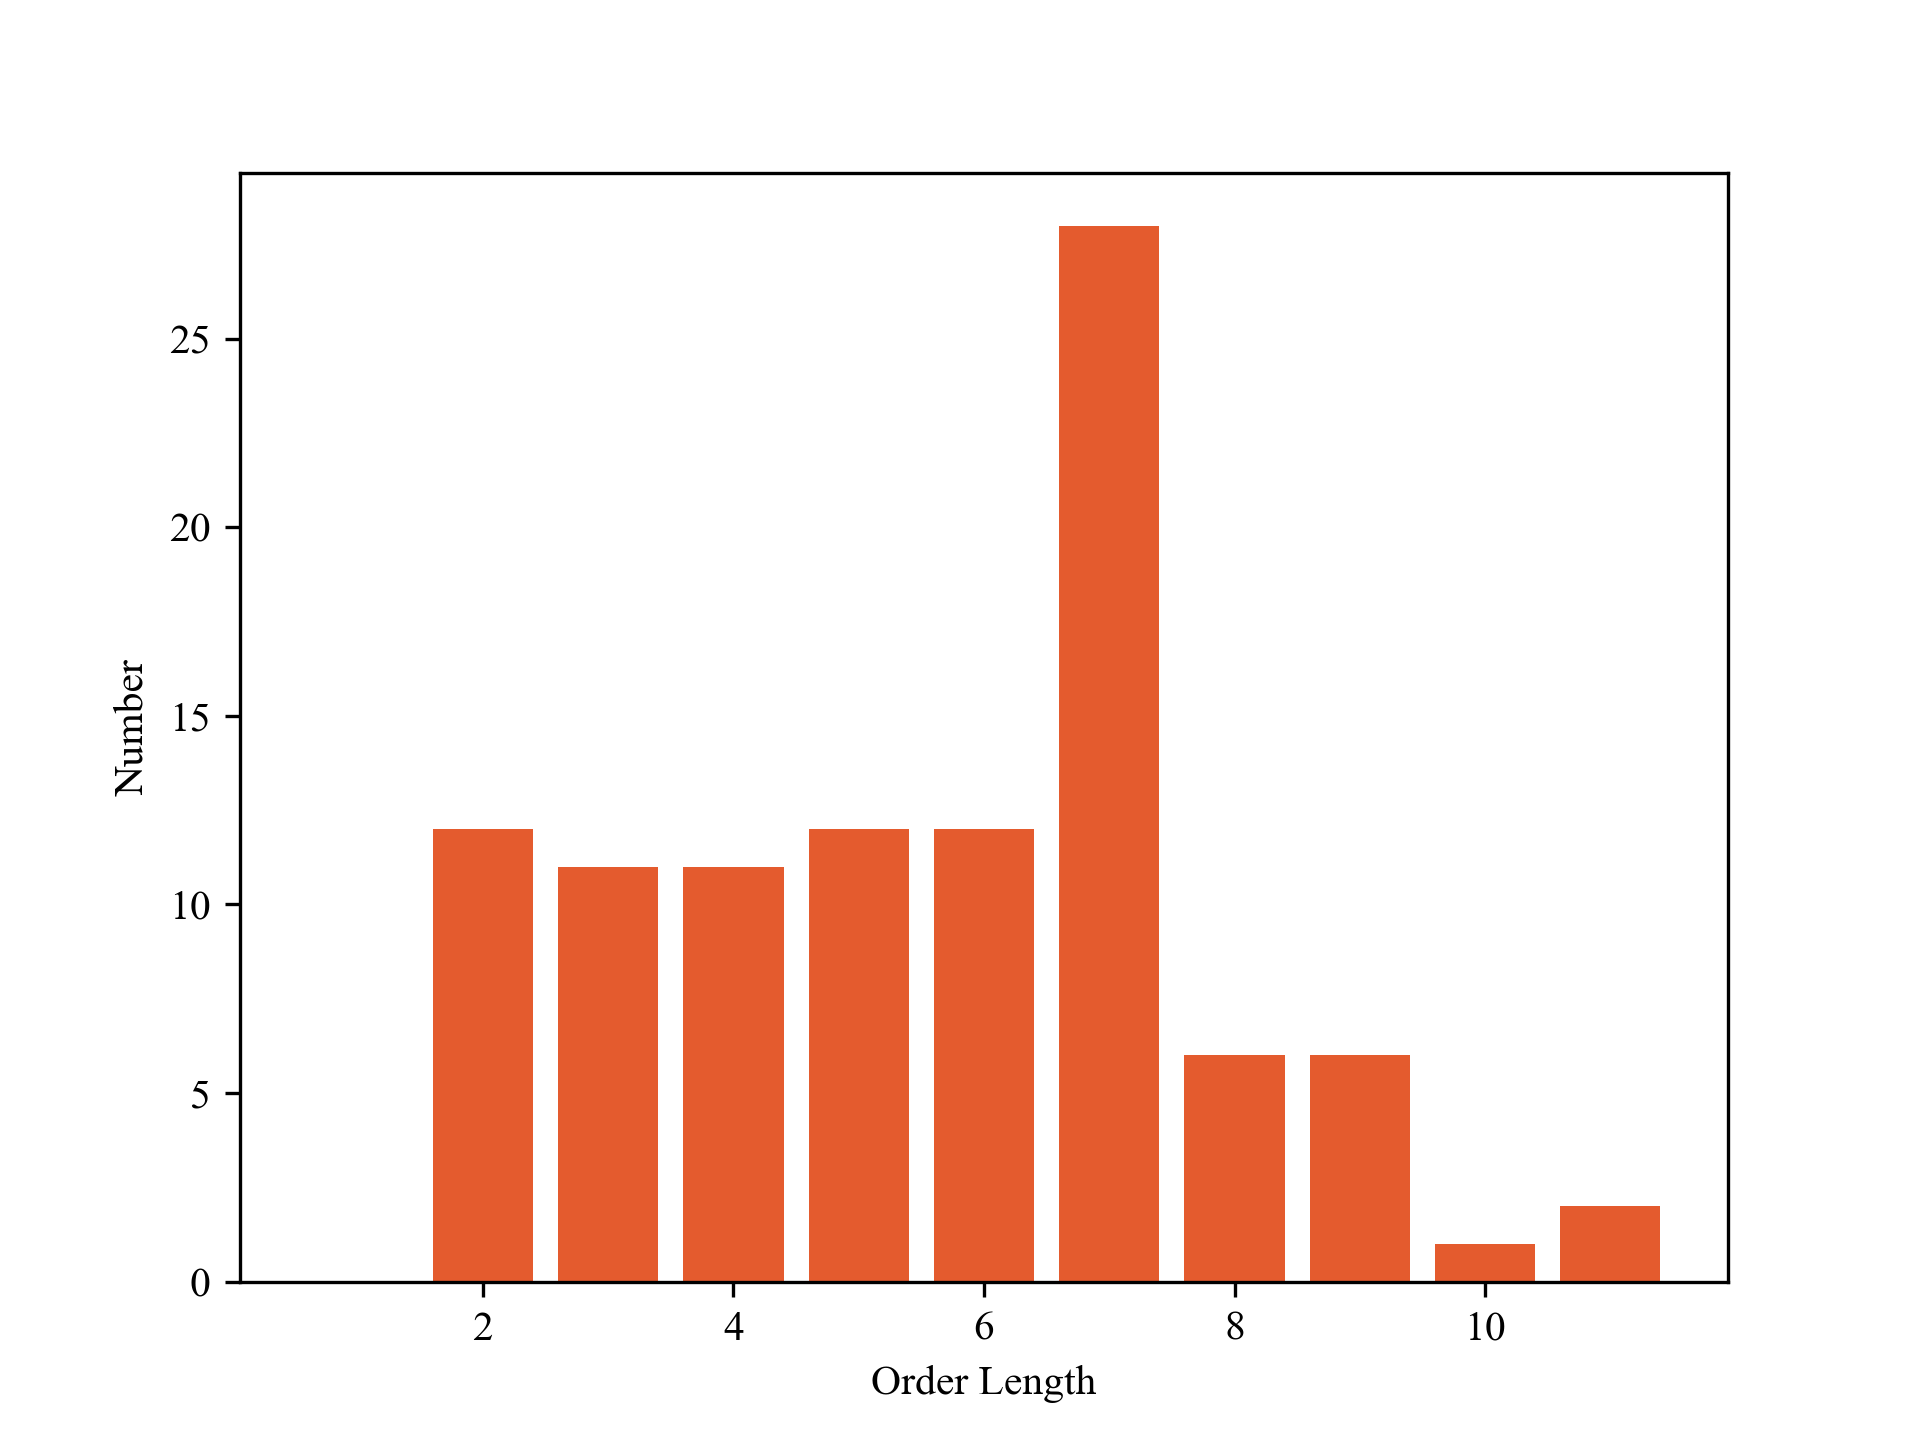
\includegraphics[scale=0.4]{orders_classification.png}
\end{figure}

智能家居的语音指令\footnote{具体内容可参见附录\ref{appendix:A}}按照不同的智能家具进行划分,各类指令的分配情况如表\ref{tab:1}所示。

\begin{table}[h]
    \caption{\label{tab:1} 智能家居语音指令数据库指令分配}
    \begin{center}
        \begin{tabular}{ccc}
            \toprule
            \textbf{指令种类} & \textbf{指令数量} & \textbf{例子} \\
            \midrule
            \textit{空调} & 20 & 打开空调、制冷、制热 \\
            \textit{门窗} & 12 & 开门、打开窗帘 \\
            \textit{照明} & 10 & 开灯、调亮灯光 \\
            \textit{风扇} & 10 & 开电风扇、一档风速 \\
            \textit{洗碗机} & 5 & 打开洗碗机 \\
            \textit{烘干机} & 8 & 打开烘干机 \\
            \textit{洗衣机} & 8 & 打开洗衣机 \\
            \textit{烤箱} & 8 & 设置烤箱温度 \\
            \textit{微波炉} & 7 & 打开微波炉\\
            \textit{热水壶} & 5 & 打开热水壶 \\
            \textit{热水器} & 4 & 开热水器 \\
            \textit{安防} & 11 & 打开防盗门 \\
            \textit{预定} & 18 & 预定洗衣机时间 \\
            \textit{定时} & 7 & 一小时 \\
            \textit{其他} & 15 & 扫地机器人开始工作 \\
            \bottomrule
        \end{tabular}
    \end{center}
\end{table}

通过合理设计语音指令文本,确保涵盖了智能家居的主要操作场景,并通过不同语速和语调的变化,提升模型对真实场景的适应能力。

\subsection{语音数据增强}

为了增加方言数据集的容量并提高识别精度,我们采用了数据增强技术。具体而言,对原始数据进行了语调、音调和音量等方面的增强。我们使用了多种数据增强技术生成多样化的数据集,例如加入随机噪声或改变音频中的音调高低。这些增强后的数据集能够有效解决原始数据量少和质量不高的问题,为模型训练提供更丰富的语音数据。

数据增强技术包括:
\begin{itemize}
    \item \textbf{时间拉伸}:调整音频的播放速度,而不改变其音调。
    \item \textbf{音量调节}:改变音频的音量大小,以模拟不同的说话音量。
    \item \textbf{背景噪声添加}:在音频中加入不同类型的背景噪声,例如白噪声、街道噪声等。
    \item \textbf{频率变换}:对音频信号进行频率变换,模拟不同的声调和发音特点。
\end{itemize}

这些数据增强方法显著提高了方言识别模型的性能,为智能家居语音指令领域的研究和应用提供了有力支持。通过多样化的数据集,模型能够更好地适应不同的语音输入,提高识别的准确性和鲁棒性。

综上所述,构建包含普通话和多种方言的智能家居语音指令数据库,并通过数据增强技术丰富数据集,是提升智能家居语音识别系统性能的关键。本研究所构建的数据库和采用的数据增强方法,将为智能家居语音指令识别领域提供重要的技术支持和实践经验。


\section{符号说明}
\begin{longtable}{ccc}
    \caption{研究中涉及的变量}\label{tab:2} \\
    \toprule
    \textbf{变量} & \textbf{含义} &\textbf{类型} \\ 
    \midrule 
    \endfirsthead

    \multicolumn{3}{c}%
    {\small{\textbf{表 \thetable{} :} 研究中涉及的变量}} 续表\\
    \toprule
    \textbf{变量} & \textbf{含义} &\textbf{类型} \\
    \midrule
    \endhead

    \bottomrule
    \endfoot

    \bottomrule
    \endlastfoot

    $\mathcal{M}$ & 普通话 & Group\\
    $\mathcal{D}$ & 目标方言 & Group\\
    $\mathcal{D}_Y$ & 义乌方言 & Group\\
    $\mathcal{D}_C$ & 粤语 & Group\\
    $\mathcal{D}_S$ & 四川方言 & Group\\
    $\mathcal{D}_H$ & 沪语 & Group\\
    $L$ & 指令数据条数 & Integer\\
    $\Xi$ & 指令数据集合 & Set\\
    $S_m(t)$ & 普通话语音指令数据 & Signal\\
    $S_d(t)$ & 目标方言语音指令数据 & Signal\\
    $M_m(t)$ & 普通话语音指令数据的梅尔倒谱系数矩阵 & Matrix\\
    $M_d(t)$ & 目标方言语音指令数据的梅尔倒谱系数矩阵 & Matrix\\
    $M_{SVD}$ & 梅尔倒谱矩阵$M$的SVD降维结果矩阵 & Matrix\\
    $\Delta t$ & 窗函数的时间间隔 & Float\\
    $\bm{v_m}$ & 普通话语音指令数据的特征向量 & Vector\\
    $\bm{v_d}$ & 目标方言语音指令数据的特征向量 & Vector\\
    $S_p(t)$ & 待预测的指令数据 & Signal\\
    $M_p(t)$ & 待预测的指令数据的梅尔倒谱系数矩阵 & Matrix\\
    $\bm{v_p}$ & 待预测的指令数据的特征向量 & Vector\\
    $\theta$ & 待预测的指令数据与普通话指令数据的夹角 & Float\\
    $\Omega$ & 目标方言映射到普通话的权重矩阵 & Matrix\\
    $E$ & 目标方言映射到普通话的误差常数矩阵 & Matrix\\
\end{longtable}

\section{语音识别方法}
\subsection{音频特征提取算法}
常用的音频特征提取算法有傅里叶变换、短时傅里叶变换、梅尔频率倒谱系数、小波变换\cite{grossmann1984decomposition}等。通过合理的算法选择,能够提升特征值的有效性,进而使识别更精准。

梅尔频率倒谱系数,(Mel-Scale Frequency Cepstral Coefficients, MFCCs)是一种在语音识别领域中运用的最为广泛的特征提取算法之一,由Davis和Mermelstein等\cite{Davis1980}在1980年提出。MFCC的提取过程模仿了人耳由于生理构造而具有的听觉特性,特别是对不同频率的声音的感知方式。人耳对频率的感知是非线性的,即对低频声音的分辨能力比高频声音要好。因此,MFCC特征的提取过程包括将频率转换到一个称为梅尔刻度(Mel scale)的尺度上,该尺度更接近人类的听觉感知。

\begin{equation}
    m = Mel(f) = 2595 \log_{10}(1+f/700)
\end{equation}

其中,$f$是频率,$m$即是对应的Mel刻度。

MFCCs的计算分为:预加重、加窗、短时傅里叶变换、计算功率谱密度、应用梅尔滤波器、离散余弦变换等步骤。最终将语音数据转化为MFCCs的特征向量,进而用于语音识别的声学模型中。

预加重的目的为消除低频率对结果的负面影响,通过高通滤波实现,根据经验,本研究中在计算MFCC时使用一阶差分方程,即:

\begin{equation}
    x'(n) = x(n) + \alpha x(n-1) 
\end{equation}

其中,$\alpha$指预加重系数。

加窗的目的为消除边界干扰,即对输入信号进行窗函数处理,如Hanning窗或Rectangular窗等,消除频谱泄露的效应。

\begin{equation}
    x_w(n) = x'(n) \cdot w(n)
\end{equation}

其中,$w(n)$为窗函数,一般有矩形窗、海明(Hamming)窗、汉宁(Hanning)窗等。本研究中使用了受到广泛认可的Hamming窗,相对于其他窗函数,Hamming窗具有更好的频谱主瓣宽度和边界衰减,而且计算更为简便。
\begin{equation}
    w(n) = H(n) = 0.54 - 0.46 \cos \left( \frac{2\pi n}{N-1} \right)
\end{equation}

傅里叶变换(Fourier Transform)是一种针对时域信号的变换。傅里叶在其著作《热的解析理论》\cite{baron2003analytical}中提出傅里叶级数,即:
\begin{equation}
    f(t) = \frac{a_0}{2} +\sum_{n=1}^{\infty} [a_n \cos(n\omega t)+b_n\sin(n\omega t)]
\end{equation}

傅里叶级数的数学意义即把一个信号转化为无数个正余弦函数之和,这是傅里叶变换的基础。
\begin{equation}
    F(\omega) = \int_{-\infty}^{\infty} f(t) \cdot e^{-j\omega t} \cdot dt
\end{equation}

其中,$f(t)$是原信号,$F(\omega)$是经过傅里叶变换后的信号。傅里叶变换是语音特征提取的基础变换,将音频信号的时域数据转化为频域数据,以方便分析频率的变化和范围。

短时傅里叶变换(Short-Time Fourier Transform, STFT)是由Gabor\cite{gabor1946theory}在1946年提出的基于傅里叶变换的音频变换方法。其原理是将语音信号转换为频率谱,它是通过对信号的离散傅里叶变换来实现的。通过将语音信号分成多个短时信号分别对其进行傅里叶变换,即对原语音信号进行短时傅里叶变换后,不会丢失时域信息,可以同时得到频域和时域的信息。
\begin{equation}
    X(m, \omega) = \sum_{n=-\infty}^{\infty} x(n) \cdot w(n-m) \cdot e^{-j\omega n}
\end{equation}

离散余弦变换(Discrete Cosine Transform, DCT)在MFCCs的计算中将通过Mel滤波器后的信号转化为最后的向量形式。
\begin{equation}
    f_m = \sum_{k=0}^{n-1} x_k \cos [\frac{\pi}{n}m(k+\frac{1}{2})]
\end{equation}

本研究使用MFCCs对每条进行语音数据的特征提取,用于语音识别的声学模型中。将对一个音频信号$S(t)$求取MFCCs的操作定义为${MFCC}(S(t))$,计算得到了时间序列上每个窗口的MFCCs特征向量,即有:
\begin{equation}
    M = MFCC(S(t)) = 
    \begin{bmatrix}
        f_{[0,\Delta t]}\\
        f_{[\frac{\Delta t}{2},\frac{3\Delta t}{2}]}\\
        f_{[\Delta t,2\Delta t]}\\
        \vdots\\
        f_{[n-1\Delta t,n\Delta t]}
    \end{bmatrix}
\end{equation}
\subsection{数据降维}
奇异值分解(Singular Value Decomposition, SVD)是矩阵分解的一种方法,是一种广泛应用的数据降维方法,通过计算出的奇异值自大到小排序,可以得出不同特征的重要程度。进而选择重要程度高的特征,实现降维。

本研究对于音频计算了其梅尔频率倒谱系数,通过奇异值分解,按特征重要程度自高向低取重要的特征,删除贡献率小的特征,排除了潜在的由于过多无关特征而导致的模型过拟合现象。

对于一个语音信号$S(t)$计算其梅尔频率倒谱系数,得到以时间序列上每个窗口的MFCCs特征向量作为行向量的矩阵$M$,即:

\begin{equation}
    M = 
    \begin{bmatrix}
        m_{1,1} & m_{1,2} & \ldots & m_{1,13} \\
        m_{2,1} & m_{2,2} & \ldots & m_{2,13} \\
        \vdots & \vdots & \ddots & \vdots \\
        m_{L,1} & m_{L,2} & \ldots & m_{L,13}\\
    \end{bmatrix}
\end{equation}

对于矩阵$M$,存在$M = U \cdot \Sigma \cdot V^T$,其中$U$是$M$的左奇异矩阵,$\Sigma$是$M$的对角矩阵,$V^T$是$M$的右奇异矩阵。其中,$\Sigma_{i,i}$为$M$的奇异值,降序排列。取奇异值排序的前$k$项,则有
\begin{equation}
    M_k = U_k \cdot \Sigma_k \cdot V^T_k
\end{equation}

其中,称$M_k$是原矩阵$M$的$k$维近似矩阵,$U_k$是$U$的前$k$列,$V_k$是$V^T$的前$k$行,$\Sigma_k$是$M$的前$k$个奇异值,$r(M_k)$代表矩阵$M_k$的秩。

\subsection{映射}
现有普通话智能家居语音指令数据集$X=\{S_{m_1}, S_{m_2}, \ldots, S_{m_L}\}$,其中$S_{m_i}$为第$i$条普通话语音指令数据;方言智能家居语音指令数据集$Y=\{S_{d_1}, S_{d_2}, \ldots, S_{d_L}\}$,其中$S_{d_i}$为第$i$条方言语音指令数据;依次通过提取MFCCs特征值、SVD奇异值分解降维等步骤,可以得到普通话智能家居语音指令特征矩阵集$\mathbb{D} = \{ M_{m_1}, M_{m_2}, \ldots, M_{m_L}\}$和方言智能家居语音指令特征矩阵集$\mathbb{M} = \{ M_{d_1}, M_{d_2}, \ldots, M_{d_L}\}$。

寻找方言集合$\mathbb{D}$ 与普通话集合$\mathbb{M}$的映射关系,简单来说,就是要找到方言矩阵和普通话矩阵之间的关系,即同一指令的方言语音特征矩阵$M_d$与普通话语音特征矩阵$M_m$之间的映射关系,即如图\ref{fig:map_easy}所示。
\begin{figure}[h]
    \caption{\label{fig:map_easy}方言和普通话映射关系示意图}
    \centering
    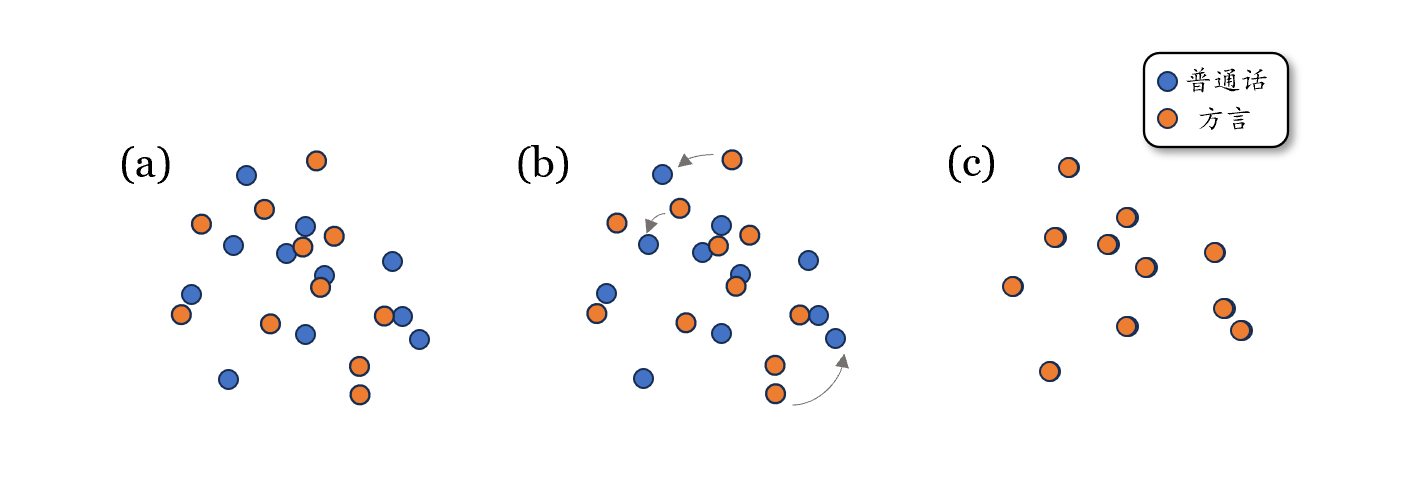
\includegraphics[scale=0.3]{Map.png}
\end{figure}

图\ref{fig:map_easy}(a)即是普通话和方言的指令对应的点在平面上的近似分布,(b)中的箭头即方言集合$\mathbb{D}$和普通话集合$\mathbb{M}$之间的映射关系,我们希望能找到这些箭头所对应的数学函数或方程,使得(a)中的元素可以完美地转化到(c)的状态。

寻找权重矩阵$\Omega_{\mathbb{D}\rightarrow \mathbb{M}}$以及误差矩阵$E_{\mathbb{D}\rightarrow \mathbb{M}}$,使其满足:
\begin{equation}
    M_m = \Omega_{\mathbb{D}\rightarrow  \mathbb{M}} \odot M_d + E_{\mathbb{D}\rightarrow \mathbb {M}}
\end{equation}

对$M_m$和$M_d$中的任意元素$m_{ij}$, 记在普通话语音指令数据集$A$中有数组$\mathbf{U}_{ij} = [m_{1_{ij}}, m_{2_{ij}}, \ldots, m_{L_{ij}}]$,方言语音指令数据集$B$中有数组$\mathbf{V}_{ij} = [d_{1_{ij}}, d_{2_{ij}}, \ldots, d_{L_{ij}}]$,$i \in \{ 1, 2, \ldots, L\}$,$j \in \{ 1, 2, \ldots, L\}$,其中,$m_{k_{ij}}$代表第$k$个矩阵$M_m$的第$i$行第$j$列元素,$d_{k_{ij}}$代表第$k$个矩阵$M_d$的第$i$行第$j$列元素。

采用回归算法,以$\mathbf{V}_{ij}$作为自变量$x$,$\mathbf{U}_{ij}$作为因变量,分别采取不同的函数进行对数据进行运算,则对元素$(i,j)$有对应的均方根误差RMSE,记为$R_{ij}$,则有均方根误差矩阵$R$代表每个元素对应均方根差的矩阵,即:
\begin{equation}
    R = \begin{bmatrix}
        R_{1,1} & R_{1,2} & \cdots & R_{1,N}\\
        R_{2,1} & R_{2,2} & \cdots & R_{2,N}\\
        \vdots & \vdots & \ddots & \vdots\\
        R_{L,1} & R_{L,2} & \cdots & R_{L,N}\\
    \end{bmatrix}
\end{equation}
记当使用函数$g(x)$作为回归函数时,其均方根误差矩阵为$R_g$。$R_g$的所有元素的平均值为$\mu_g$,即:
\begin{equation}
    \mu_g = \frac{1}{NL}\sum_{i=1}^{L} \sum_{j=1}^{N} R_{g_{ij}}
\end{equation}

对于不同函数$g(x)$的均方根误差矩阵$R_g$,我们有不同的$\mu_g$,我们需要找到最小的$\mu_g$,以其对应的函数作为回归函数,即:
\begin{equation}
    \mathop{\min}_{g} \mu_g = \frac{1}{NL}\sum_{i=1}^{L} \sum_{j=1}^{N} R_{g_{ij}}
\end{equation}

以下以一元线性回归为例,即:
\begin{equation}
    \hat{y} = \beta_0 + \beta_1 x
\end{equation}
解得:
\begin{equation}
    \left\{ 
    \begin{aligned}
           \beta_1 &= \frac{\sum_{k=1}^{L} (\mathbf{V}_{{ij}_k}-\overline{\mathbf{V}_{ij}}) (\mathbf{U}_{{ij}_k}-\overline{\mathbf{U}_{ij}})}{\sum_{k=1}^{L} (\mathbf{V}_{{ij}_k}-\overline{\mathbf{V}_{ij}})^2}\\
        \beta_0 &= \overline{\mathbf{U}_{ij}}-\beta_1 \overline{\mathbf{V}_{ij}}
    \end{aligned}
    \right.
\end{equation}

于是对于元素$(i,j)$,我们有$\omega_{ij} = \beta_1$, $\varepsilon_{ij} = \beta_0$。因此我们找到的目标方言集合$\mathbb{D}$与普通话集合$\mathbb{M}$的映射关系,即权重矩阵$\Omega$和误差补充矩阵$E$。

\begin{equation}
    \Omega = \begin{bmatrix}
        \omega_{11} & \omega_{12} & \cdots & \omega_{1N}\\
        \omega_{21} & \omega_{22} & \cdots & \omega_{2N}\\
        \vdots & \vdots & \ddots & \vdots \\
        \omega_{L1} & \omega_{L2} & \cdots & \omega_{LN}
    \end{bmatrix}, 
    E = \begin{bmatrix}
        \varepsilon_{11} & \varepsilon_{12} & \cdots & \varepsilon_{1N}\\
        \varepsilon_{21} & \varepsilon_{22} & \cdots & \varepsilon_{2N}\\
        \vdots & \vdots & \ddots & \vdots \\
        \varepsilon_{L1} & \varepsilon_{L2} & \cdots & \varepsilon_{LN}
    \end{bmatrix}
\end{equation}

\subsection{预测}
现有普通话智能家居语音指令数据库,包含一系列语音音频数据$D_i(t)$, $i = 1, 2, \ldots, L$。

对$D_i(t), i\in \{1,2,\ldots, L\}$,有$M_i = MFCC(D_i(t))$。

通过SVD分解降维得到$M_{SVD_i}$。

有一条待预测的音频指令数据,记为$S_p(t)$,通过梅尔频率倒谱系数的计算,提取得到矩阵$M_p$,即:
\begin{equation}
    M_p = MFCC(S_p(t))
\end{equation}

进一步得到矩阵$M_{SVD_p}$。

通过映射过程,将符合方言特征的矩阵$M_{SVD_p}$转化为符合普通话特征的矩阵。以下以一元线性回归为例,即对于$m_{ij}$可映射为$\omega_{ij}m_{ij}+\varepsilon_{ij}$。
\begin{equation}
\begin{aligned}
    D_p &= F(M_{SVD_p}) = \Omega_{\mathbb{D}\rightarrow  \mathbb{M}} \odot M_{SVD_p} + E_{\mathbb{D}\rightarrow \mathbb{M}} \\
    &= \begin{bmatrix}
        \omega_{1,1} & \omega_{1,2} & \cdots & \omega_{1,N} \\
        \omega_{2,1} & \omega_{2,2} & \cdots & \omega_{2,N} \\
        \vdots & \vdots & \ddots & \vdots \\
        \omega_{L,1} & \omega_{L,2} & \cdots & \omega_{L,N}\\
    \end{bmatrix} \odot \begin{bmatrix}
        m_{1,1} & m_{1,2} & \cdots & m_{1,N} \\
        m_{2,1} & m_{2,2} & \cdots & m_{2,N} \\
        \vdots & \vdots & \ddots & \vdots \\
        m_{L,1} & m_{L,2} & \cdots & m_{L,N}\\
    \end{bmatrix} + \begin{bmatrix}
        \varepsilon_{1,1} & \varepsilon_{1,2} & \cdots & \varepsilon_{1,N} \\
        \varepsilon_{2,1} & \varepsilon_{2,2} & \cdots & \varepsilon_{2,N} \\
        \vdots & \vdots & \ddots & \vdots \\
        \varepsilon_{L,1} & \varepsilon_{L,2} & \cdots & \varepsilon_{L,N}\\
    \end{bmatrix}\\
    &= \begin{bmatrix}
        \omega_{1,1}m_{1,1}+\varepsilon_{1,1} & \omega_{1,2}m_{1,2}+\varepsilon_{1,2} & \cdots & \omega_{1,N}m_{1,N}+\varepsilon_{1,N} \\
        \omega_{2,1}m_{2,1}+\varepsilon_{2,1} & \omega_{2,2}m_{2,2}+\varepsilon_{2,2} & \cdots & \omega_{2,N}m_{2,N}+\varepsilon_{2,N} \\
        \vdots & \vdots & \ddots & \vdots \\
        \omega_{L,1}m_{L,1}+\varepsilon_{L,1} & \omega_{L,2}m_{L,2}+\varepsilon_{L,2} & \cdots & \omega_{L,N}m_{L,N}+\varepsilon_{L,N}\\
    \end{bmatrix}
\end{aligned}
\end{equation}

对于$D_p$和$M_{SVD_i}, i \in \{ 1,2,\ldots, L\}$, 计算对应行向量的余弦相似度。即:
\begin{equation}
    \cos \theta_{pi_{j}} = \cos \langle \bm{v_{p_j}},\bm{v_{i_j}} \rangle = \frac{\bm{v_{p_j}} \cdot \bm{v_{i_j}}}{|\bm{v_{p_j}}||\bm{v_{i_j}}|}
\end{equation}

其中,$\bm{v_{p_j}}$和$\bm{v_{i_j}}$分别为$D_p$和$M_{SVD_i}$的第$j$行。

当$\theta$越小,意味着两个向量之间的余弦相似度越大。因而:
\begin{equation}
    \mathop{\min}_{i} ~~\overline{\theta} = \dfrac{1}{L} \sum_{j=1}^{L} \theta_{pi_{j}}, ~~i \in \{1,2,\ldots, L\}
\end{equation}

有$\overline{\theta_{pk}} = \theta_{min}$, 则对应的普通话指令为$S_k(t)$。
\section{结果与讨论}
\subsection{映射关系矩阵}
通过计算数据库中方言$\mathcal{D}$和普通话$\mathcal{M}$的MFCCs矩阵和对应的SVD矩阵,并使用不同回归函数进行映射关系矩阵的计算。其均方根误差矩阵$R$的热力图及其平均均方根误差$\mu$如图所示。
\begin{figure}[h]
    \caption{\label{fig:heatmap_mu}不同回归函数的均方根误差矩阵热力图}
    \centering
    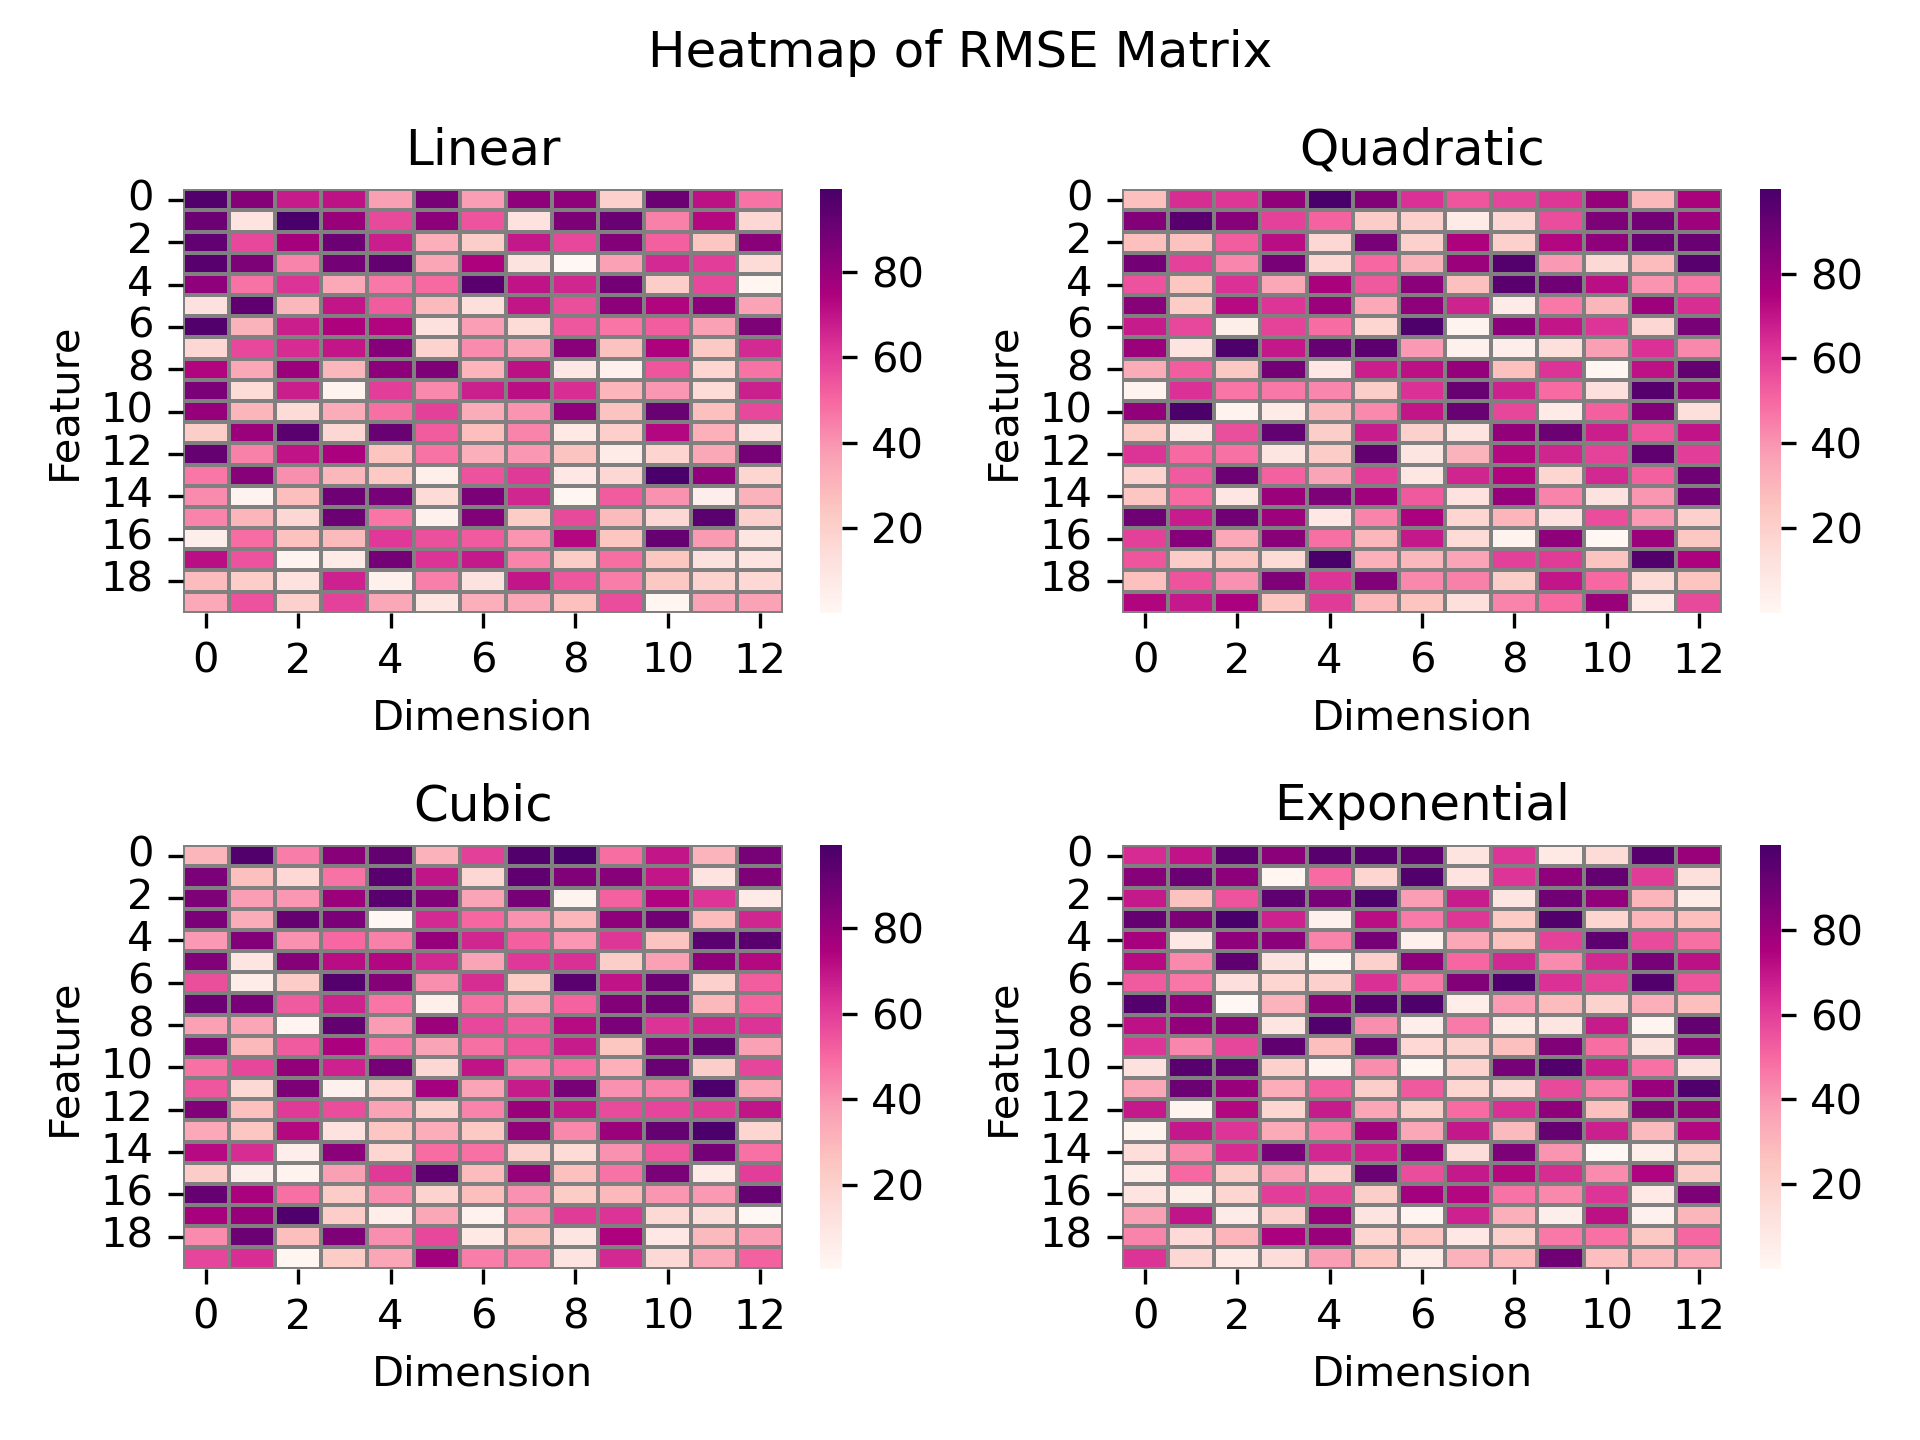
\includegraphics[scale=0.6]{RMatrix.png}
\end{figure}

通过对比,可以发现不同的回归函数所对应的均方根误差矩阵的平均均方根误差相差不大,为避免过拟合的行为出现,在此采用最基础的一元线性回归模型。浙江义乌话$\mathcal{D}_Y$和普通话$\mathcal{M}$之间的映射关系权重矩阵所对应的热力图如图\ref{fig:heatmap_weight}所示。
\begin{figure}[h]
    \caption{\label{fig:heatmap_weight} $\mathcal{D}_Y$与$\mathcal{M}$权重矩阵热力图}
    \centering
    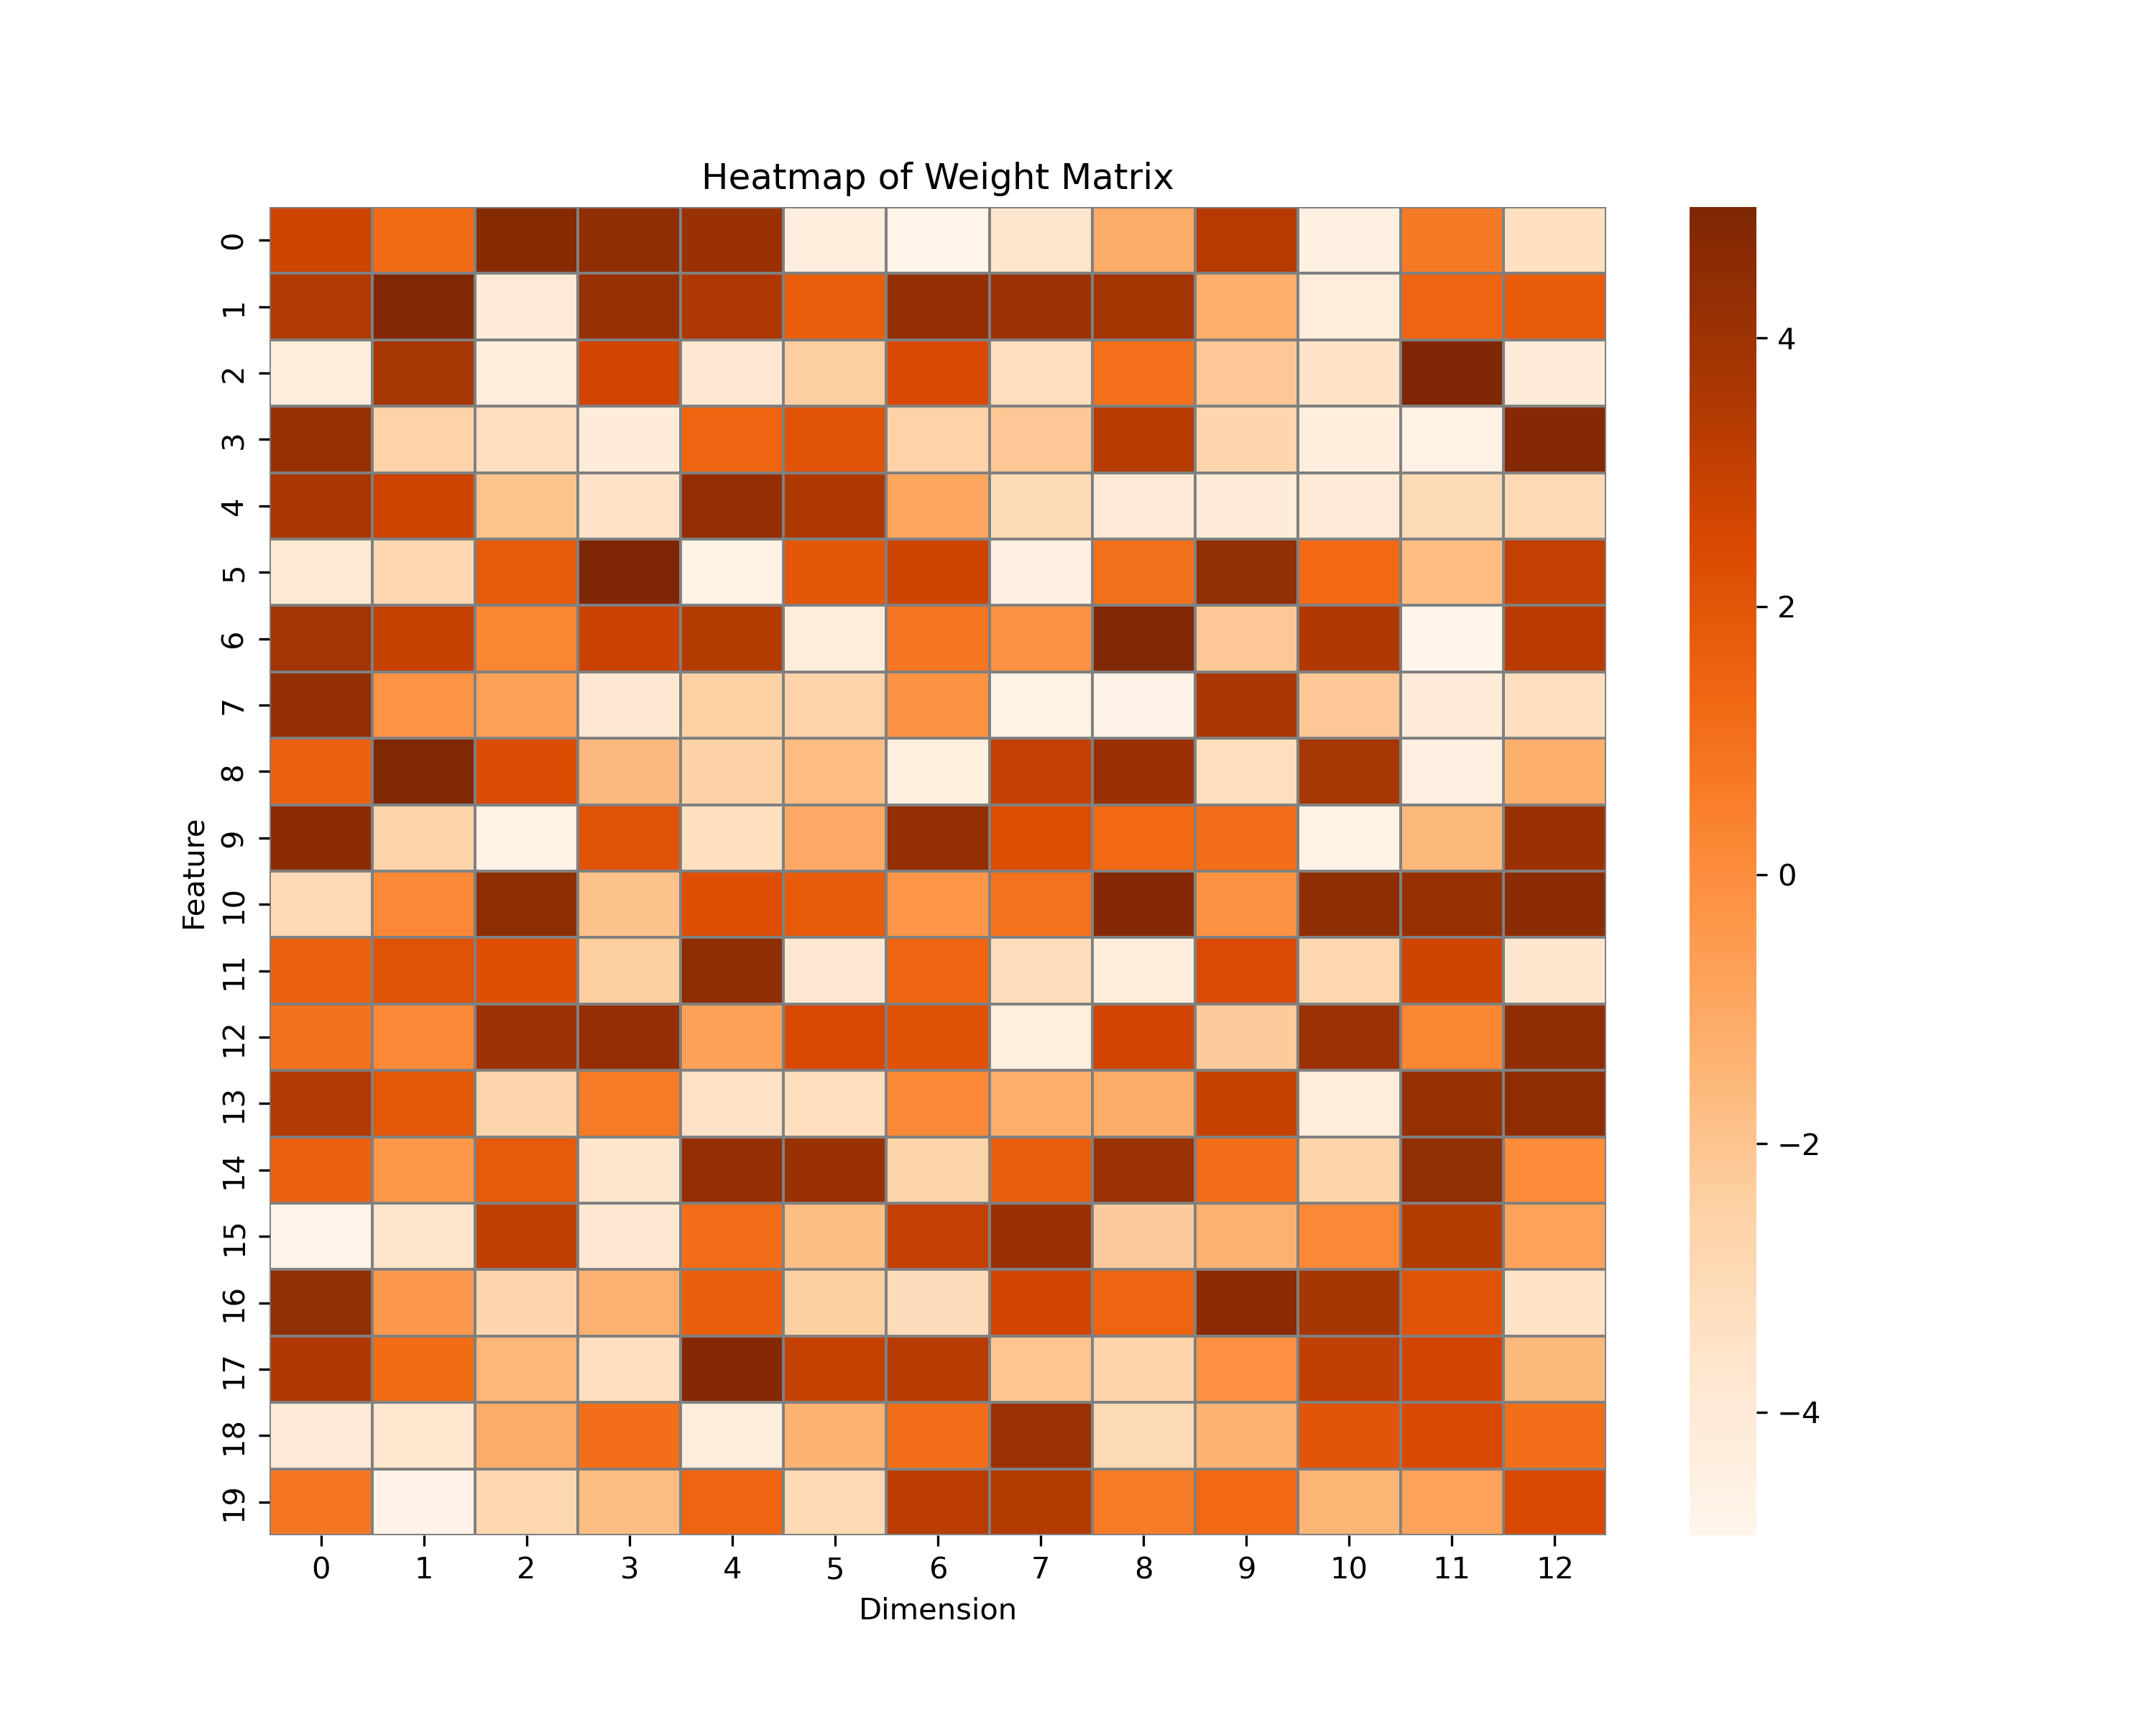
\includegraphics[scale=0.35]{Weight_Matrix_Heatmap.png}
\end{figure}

同样地,通过一元线性回归,我们还得出了映射关系的常数误差矩阵,其所对应的热力图如图\ref{fig:heatmap_constant}所示。
\begin{figure}[h]
    \caption{\label{fig:heatmap_constant} $\mathcal{D}_Y$与$\mathcal{M}$常数误差矩阵热力图}
    \centering
    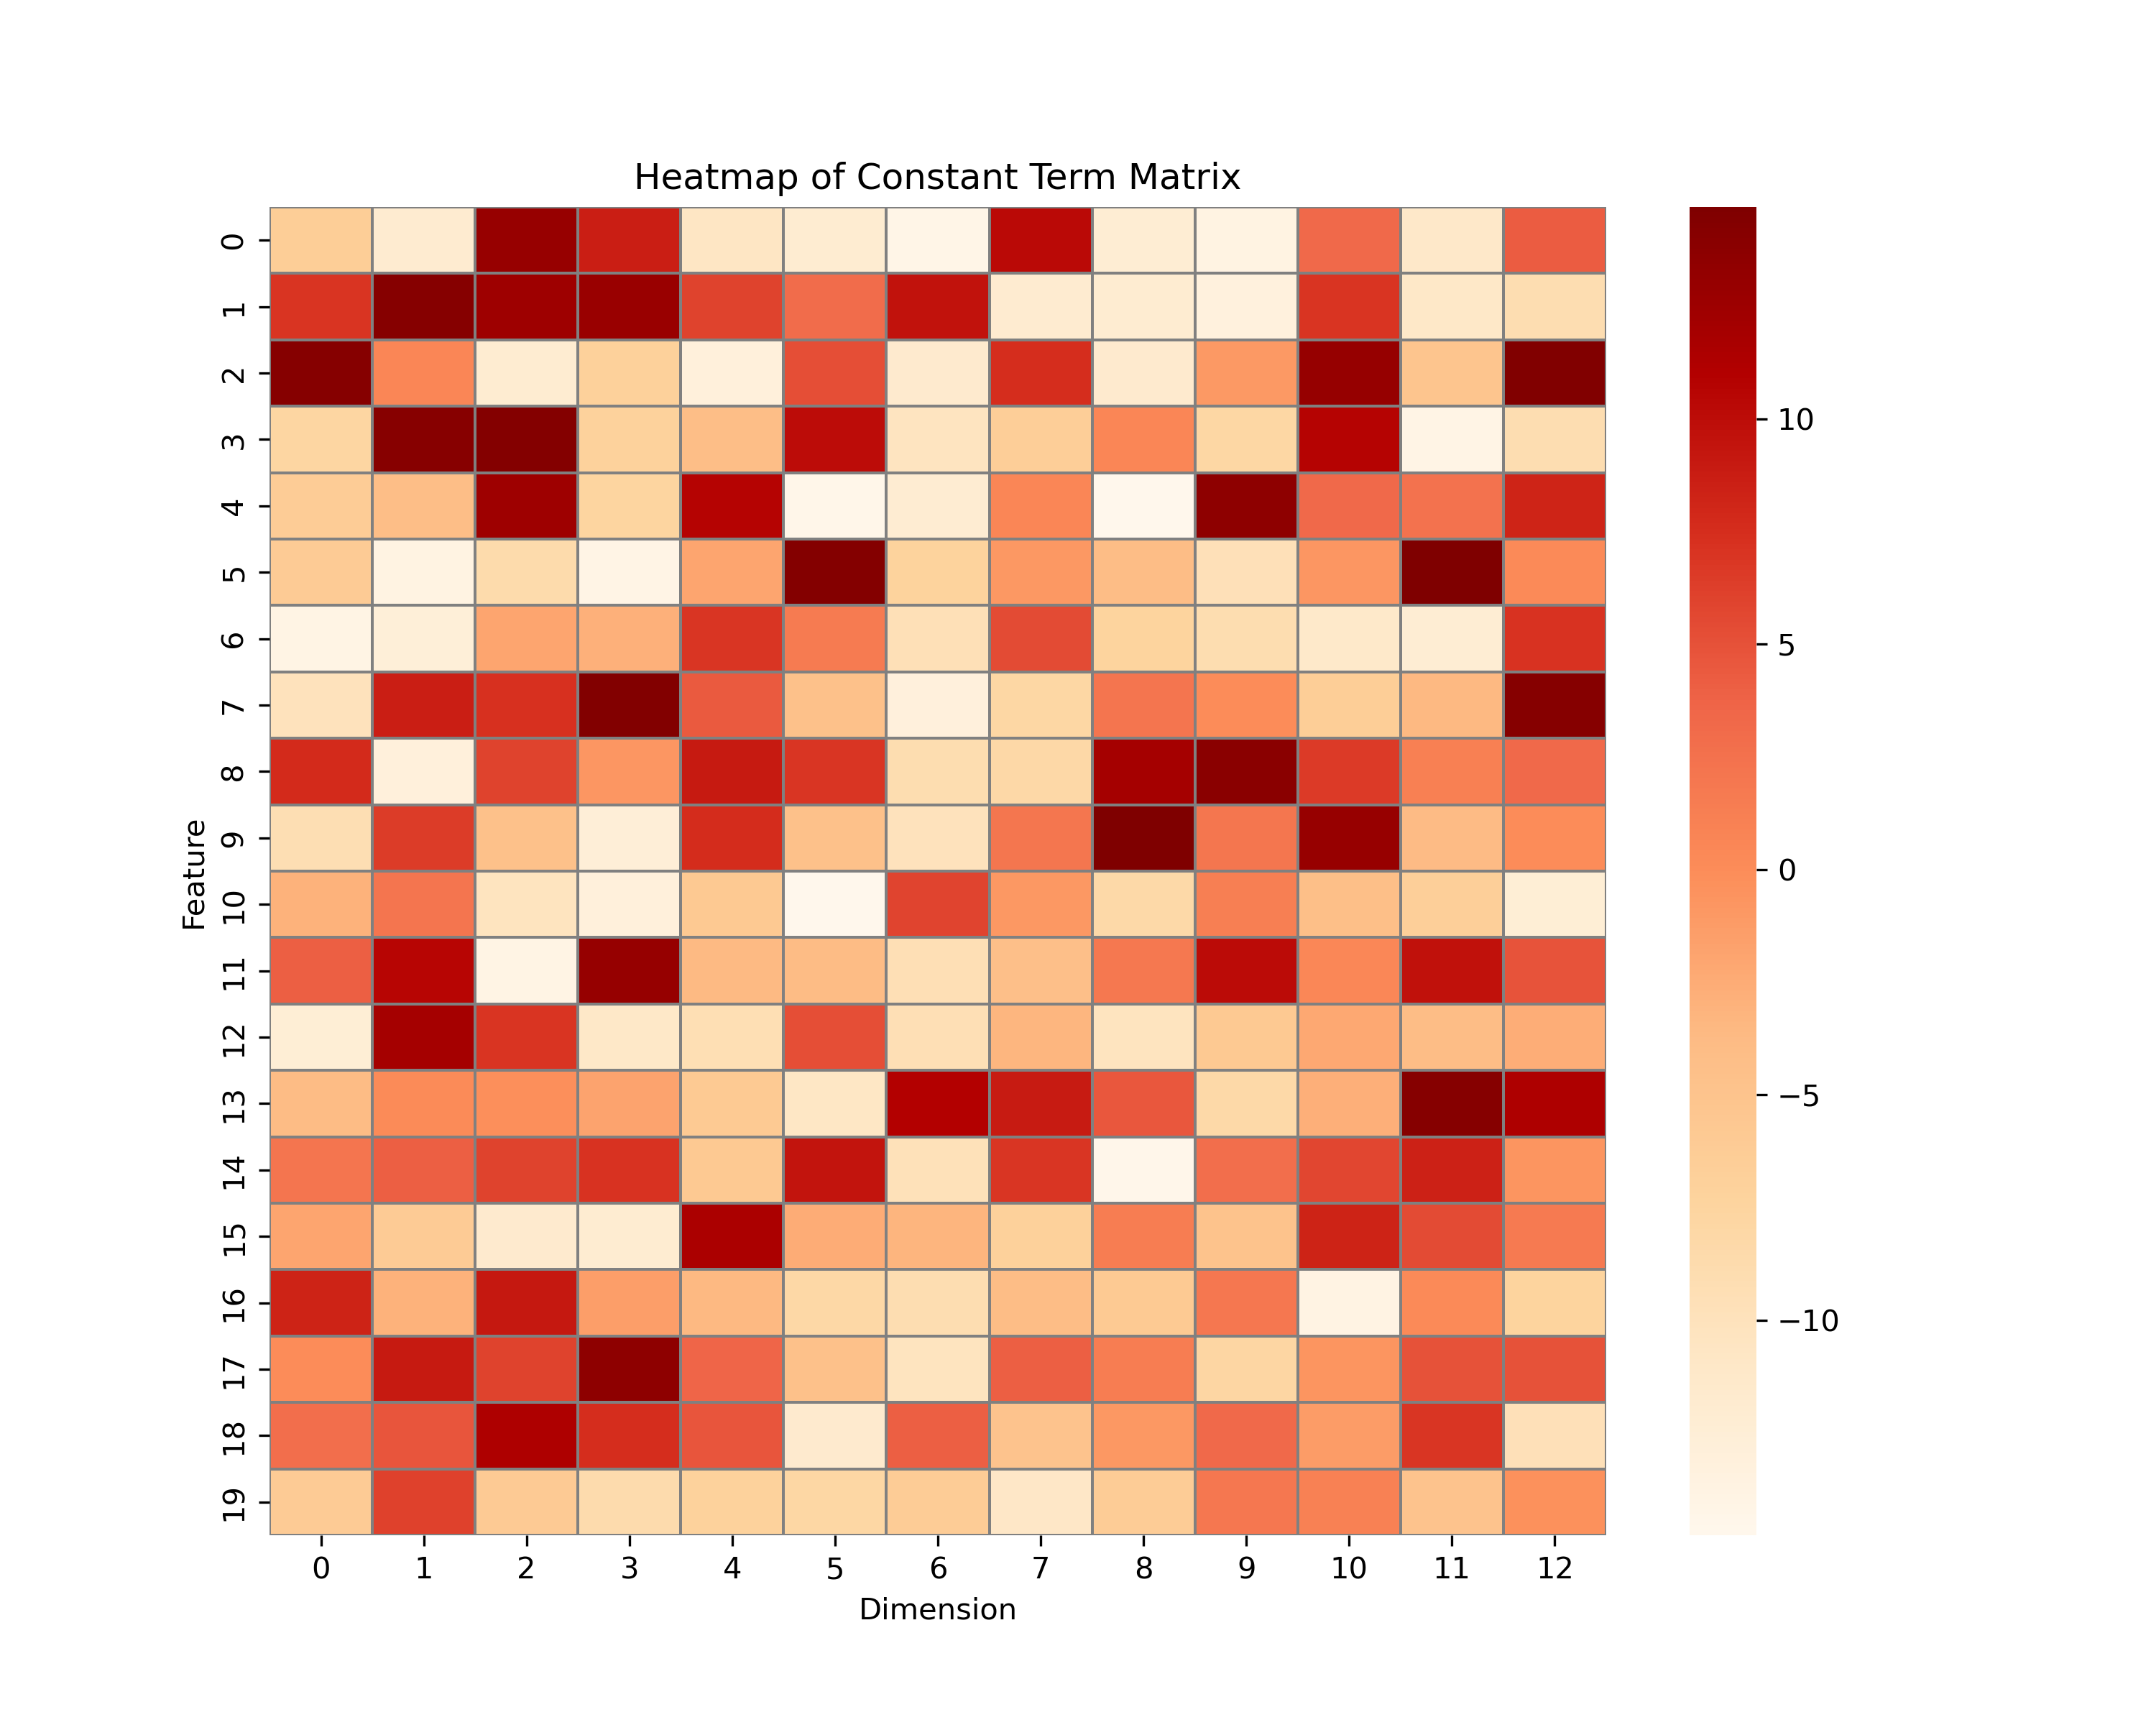
\includegraphics[scale=0.35]{Error_Matrix_Heatmap.png}
\end{figure}

通过图\ref{fig:heatmap_weight}和图\ref{fig:heatmap_constant}我们可以发现,其权重的分布是符合由奇异值分解而得出的特征的相对重要程度的,这也应证了模型的可靠性。
\subsection{转换准确率}
随机抽取每个字数的指令各2个(不足两个者全取)对模型进行测试,计算不同方言不同指令转换的准确率,通过计算概率表示,如表\ref{tab:3}所示。
\begin{table}[h]
    \caption{\label{tab:3} 各方言不同指令转换概率列表}
    \begin{center}
        \begin{tabular}{cccc}
            \toprule
            本意 & 沪语 & 四川话 & 浙江义乌话\\
            \midrule
            开门 & \makecell{开门 76.8\%\\开灯 15.4\%\\开窗 4.6\%} & \makecell{开门 82.8\%\\ 开灯 7.4\%\\ 开窗 4.6\%} & \makecell{开门 70.2\%\\ 开灯 18.7\%\\ 开窗 2.4\%}\\
            开灯 & \makecell{开灯 66.5\% \\ 开门 25.8\% \\ 开窗 0.8\%} & \makecell{开灯 83.9\% \\ 开门 6.1\% \\ 开窗 0.8\%} &\makecell{开灯 72.2\% \\ 开门 17.8\% \\ 开窗 0.8\%}\\
            开电风扇 & \makecell{开电风扇 69.7\% \\ 关电风扇 26.2\% \\ 开热水器 1.5\%} & \makecell{开电风扇88.3\% \\ 关电风扇 8.2\% \\ 开热水器 0.6\%} & \makecell{开电风扇 70.0\% \\ 关电风扇 19.0\% \\ 开热水器 0.6\%}\\
            三小时 & \makecell{三小时 62.5\% \\ 二小时 30.0\% \\ 一小时 1.1\%} & \makecell{三小时 89\% \\ 二小时 9\% \\ 四小时 0.1\%} & \makecell{三小时 70.4\% \\ 二小时 15.2\% \\ 一小时 8.6\%}\\
            预定洗碗机时间 & \makecell{预定洗衣机时间 52.5\% \\ 预定洗碗机时间 46.5\% \\ 开启洗碗机 0.5\%} & \makecell{预定洗碗机时间 93.3\% \\ 预定洗衣机时间 6.2\% \\ 开启洗碗机 0.2\%} & \makecell{预定洗衣机时间 70.1\% \\ 预定洗碗机时间 14.3\% \\ 开启洗碗机 2.4\%}\\
            \bottomrule
        \end{tabular}
    \end{center}
\end{table}

从表\ref{tab:3}可以看出,使用该方法预测具有可行性。比对不同方言的识别准确度,可以看出四川话的正确转换概率高,而浙江义乌话和沪语相对准确率低,这反映了四川话的吐字更为接近普通话的特点,而沪语和浙江义乌话属于吴语,相对发音不清楚,且存在入声、变声等特点。
\subsection{讨论}
在本研究中,我们开发并验证了一个低成本普惠型智能家居方言指令转换器。以下是对研究结果的深入讨论:

\subsubsection{映射关系矩阵的有效性}

通过对梅尔频率倒谱系数(MFCCs)的分析,我们构建了映射关系矩阵,包括映射关系权重矩阵 \( \Omega \) 和映射关系常数误差矩阵 \( E \)。实验结果表明,所提出的方法能够有效捕捉并转换方言指令,使得智能家居系统能够准确识别和执行相应的操作。然而,在不同方言之间,映射关系矩阵的准确性存在差异。这表明,不同方言的声学特征差异显著,未来可以通过进一步优化这些矩阵来提高对更多方言的识别精度。

\subsubsection{回归函数选择}

我们测试了多种回归函数,最终选择了一元线性回归模型。原因在于,在比较均方根误差(RMSE)后发现,复杂模型并未显著提高精度,反而增加了过拟合的风险。采用最简单的一元线性回归模型不仅能有效避免过拟合,还能保证模型的可解释性和计算效率。这种选择对低成本设备尤为重要,因为计算资源有限,简单模型在实际应用中更具可行性。

\section{结论}
\subsection{优点}
\begin{enumerate}
    \item 本研究提出了一种利用计算对应特征向量余弦距离的方式来识别智能家居方言语音指令,使得语音识别在保证一定准确率的情况下减少了算力的消耗以及对于大数据的需求。
    \item 本研究具有很大的发展空间和应用前景,能在日常生活中做到对于智能家居方言语音指令的识别,方便智能家居的方言用户使用语音控制智能家居设备。
    \item 本研究降低了方言识别的成本,设计了一个低成本普惠型的方言指令转换系统 
\end{enumerate}
\subsection{缺点}
\begin{enumerate}
    \item 本研究受限于经费、人员等无法收集到全面的数据,只能以部分数据再增强的方式搭建数据库,这样使得我们的数据单一,可靠性不足
    \item 本研究针对于研究方言语音指令数据,其可拓展性不强,模型很难泛化至其他领域。
\end{enumerate}
\subsection{展望}
\begin{enumerate}
    \item 未来收集更多方面的数据,加强模型的鲁棒性
    \item 设计了一个方言语音指令转换器,应用于实际生活,帮助方言使用者打破语言障碍,更好地利用语音识别系统来控制智能家居设备。 
\end{enumerate}
\newpage
\section*{参考文献}
\addcontentsline{toc}{section}{参考文献}
\bibliography{D:\\TaoLi\\Projects\\DialectTranslation\\Paper\\References}
\newpage
\appendix
\label{appendix:A}
\begin{table}[H]
    \begin{tabularx}{\linewidth}{cX}
        \toprule
        指令种类 & 指令内容\\
        \midrule
        \textbf{空调} & 开空调,关空调,一档风,二档风,三档风,静音,睡眠,制冷,制热,升温,降温,预定空调时间,自动模式,节能模式,除湿模式,加湿模式,风速自动,风向上方,风向下方,风向左右摆动\\
        \textbf{照明} & 开灯,关灯,调整家居设备亮度,切换家居设备颜色,调暗灯光,调亮灯光,切换到阅读模式,切换到夜灯模式,开启氛围灯,关闭氛围灯\\
        \textbf{门窗} & 开门,关门,打开窗帘,关闭窗帘,调整窗帘开合程度,打开窗户,调整窗户开启程度,打开门窗传感器,关闭门窗传感器,检查门窗状态,开启窗户通风,关闭窗户通风,设置窗帘定时开合\\
        \textbf{风扇} & 开电风扇,关电风扇,摇头,停止摇头,一档风速,二档风速,三档风速,自动模式,睡眠模式,定时关风扇\\
        \textbf{热水器} & 开热水器,关热水器,调整热水器温度,定时关热水器\\
        \textbf{热水壶} & 打开热水壶,关闭热水壶,设置热水壶温度,保温模式,快速烧水模式\\
        \textbf{烤箱} & 打开烤箱,关闭烤箱,设置烤箱温度,上火模式,下火模式,预热烤箱,关闭预热,定时关烤箱\\
        \textbf{微波炉} & 打开微波炉,关闭微波炉,设置微波炉加热时间,解冻模式,烘烤模式,快速加热模式,定时关微波炉\\
        \textbf{洗碗机} & 打开洗碗机,关闭洗碗机,启动洗碗机清洗,取消洗碗机清洗,定时关洗碗机\\
        \textbf{洗衣机} & 打开洗衣机,关闭洗衣机,启动洗衣机洗涤,取消洗衣机洗涤,快速洗模式,强力洗模式,节能洗模式,定时关洗衣机\\
        \textbf{烘干机} & 打开烘干机,关闭烘干机,启动烘干机烘干,取消烘干机烘干,快速烘干模式,强力烘干模式,节能烘干模式,定时关烘干机\\
        \textbf{安防} & 打开门铃摄像头,关闭门铃摄像头,查看摄像头画面,控制安防摄像头开始录像,控制安防摄像头停止录像,查看录像回放,打开防盗传感器,关闭防盗传感器,打开烟雾报警器, 关闭烟雾报警器, 检查烟雾报警器状态\\
        \textbf{其他家具} & 扫地机器人开始工作,扫地机器人回充,打开新风系统,关闭新风系统,调整新风系统风速,打开除湿器,关闭除湿器,调整除湿器湿度,打开空气净化器,关闭空气净化器,调整空气净化器模式,打开地暖,关闭地暖,调整地暖温度,控制智能插座连接设备\\
        \textbf{预定} & 预定空调时间,预定洗衣机时间,预定微波炉时间,预定烤箱时间,预定洗碗机时间,预定烘干机时间,预定冰箱时间,预定空气净化器时间,预定扫地机器人时间, 预定电视时间, 预定热水器时间, 预定窗帘时间, 预定智能插座时间, 预定音响时间, 预定除湿器时间, 预定加湿器时间, 预定电动窗时间, 预定智能锁时间\\
        \textbf{定时} & 一小时,两小时,三小时,四小时,半小时,十分钟,一天\\
        \bottomrule
    \end{tabularx}
\end{table}
\end{document}